\documentclass[12pt]{article}

\usepackage{amsmath}
\usepackage{amssymb}
\usepackage{epsfig}
\usepackage{epstopdf}
\usepackage{algorithm}
\usepackage{algpseudocode}
\usepackage{amsfonts}
\usepackage{mathtools}
\usepackage{upgreek}
\usepackage{tikz}
\usepackage{verbatim}

\usepackage{multirow}
\usepackage[T1]{fontenc}
\usepackage{beramono}
\usepackage{listings}
\usepackage{xcolor}
\definecolor{backcolour}{rgb}{0.95,0.95,0.92}

\lstdefinelanguage{Julia}%
{morekeywords={abstract,break,case,catch,const,continue,do,else,elseif,%
		end,export,false,for,function,immutable,import,importall,if,in,%
		macro,module,otherwise,quote,return,switch,true,try,type,typealias,%
		using,while},%
	sensitive=true,%
	morecomment=[l]\#,%
	morecomment=[n]{\#=}{=\#},%
	morestring=[s]{"}{"},%
	morestring=[m]{'}{'},%
}[keywords,comments,strings]%

\lstset{%
	language         = Julia,
	keywordstyle     = \bfseries\color{blue},
	stringstyle      = \color{magenta},
	commentstyle     = \color{gray},
	backgroundcolor= \color{backcolour}, 
	basicstyle=\footnotesize,
	showstringspaces = false,               
	numbers=left,                    
	numbersep=5pt,                 
	tabsize=4,
	frame=single,
	breaklines=true,
	postbreak=\raisebox{0ex}[0ex][0ex]{\ensuremath{\color{red}\hookrightarrow\space}}
}
\lstset{
	frame=single,
	breaklines=true,
	postbreak=\raisebox{0ex}[0ex][0ex]{\ensuremath{\color{red}\hookrightarrow\space}}
}


\begin{document}
	
	\title{CSCE 686 Homework 6 - SCP Heuristics}
	\author{Jon Knapp and Justin Fletcher}
	\maketitle
	
	\section{SCP Heuristic Design and Development [a, b]} \label{scn:design}
	
	In this section, we apply the disciplined design process advocated in \cite{ClassNotes686} to construct the algorithms fundamental to the Set Covering Problem (SCP). Additionally, we introduce three heuristics to the algorithm with the goal of reducing the search number of states which must be visited.
	
	\subsection{Problem Domain Description: SCP}
	Given a set of elements: $E=\{e_1,...,e_n\}$, a family of subsets, $\{S_1,...,S_m\}\subseteq 2^E$, and weights $w_j \geq 0$ for each $j\in\{1,...,m\}$, the SCP is defined by the following formula:
	
	\begin{align*}
	I \subseteq \{1,...,m\} \min \sum_{J \in I} w_j \\
	\:s.t.\: \bigcup_{J \in I} S_j = E
	\end{align*}
	
	
	The input domain of the problem, which is a set of elements, $E$, can be specified by a set. The family of sets, $S$, is a set of sets, where each subset contains elements $E^\prime$ and cost $c$. Formally:
	
	\begin{itemize}
		\item Input Domain $D_i$: A set of elements, E, and a set of sets. 
		\begin{itemize}
			\item E: Elements
			\item S($E^\prime$, c): Set of sets
			\begin{itemize}
				\item $E^\prime$: Set of elements where $E^\prime \in E$
				\item c: Cost of set
			\end{itemize}
		\end{itemize}	
		\item Output Domain $D_o$: A Set of sets, $B$, such that $B \in S$, and $B$ satisfies set minimum covering property. 
		
		\item Input Function $I(E, S)$: Determines if the input conditions on the input $E$ and $S$ are satisfied. The required input conditions for this domain is that, for all $S(E^\prime, c)$, $E^\prime \in E$.
		\item Output Function: $O(B)$: Determines if the output conditions are met. The conditions are given met when:
		\begin{align*}
		I \subseteq \{1,...,m\} \min \sum_{J \in I} w_j \\
		\:s.t.\: \bigcup_{J \in I} S_j = E
		\end{align*}
		
	\end{itemize}
	
	\subsection{Problem Domain and Algorithm Domain Integration}
	
	The algorithm domain to which the SCP problem will be mapped in this work is the global search via depth-first search with backtracking (GS/DFS/BT) algorithm. Thus, the algorithm domain used in this work is that of GS/DFS/BT, which is described in \cite{ClassNotes686}. In order to use this algorithm to solve the SCP problem, the SCP domain must be mapped to the GS/DFS/BT domain. This integration is accomplished as follows:
	
	\begin{itemize}
		\item GS/DFS/BT Basic Search Constructs
		\begin{itemize}
			\item \textbf{initialization($D_i$)}: Initializes $T$, where $T$ is a tableau. $T$ consists of $M$ blocks of columns, one for each $e_k$ of $E$. The $k$th block will consist of the sets of $S$ that cover $e_k$, but do not contain lower numbered elements $e_1,...,e_{k-1}$.	
			\item \textbf{next-state-generator($D_i$)}: Returns $B$, where $B \in S$.
			\item \textbf{selection($D_i$)}: Returns $b$ where $b \in S$. Generally, the specific set chosen is selected from a block of $T$ in such a way as to maximize the coverage of the elements $E$. In the case of SCP, we require that all elements $E$ are covered and that the solution is the minimum cover for $E$.
			\item \textbf{feasibility}: Returns a Boolean, which is true if, for some $b \subset S$, $E$ is covered and is false otherwise.
			\item \textbf{solution($B$, $z$)}: Returns a Boolean which is true if $S$ covers $E$ and is the minimum cover of $E$, i.e. $z$ is minimized.
			\item \textbf{objective}:Returns a set $D_o$, which in this algorithm is a minimum cover of $E$.
		\end{itemize}
		\item Delay Termination: Because the previous GS/DFS/BT search only finds a minimal set cover, rather than a minimum set cover, we must prevent the algorithm from terminating until all covering sets have been either implicitly or explicitly examined.
		\begin{itemize}
			\item In some as yet undefined loop, iterate finding all minimal set covers possible in the problem instance.
			\item Repeat the GS/DFS/BT search for SCP, avoiding duplication where possible.
		\end{itemize}
	\end{itemize}
	
	\subsection{Algorithm Domain Specification Refinement}
	
	
	In order to further refine this design, in pursuit of executable code, we must disambiguate several operations. We define a candidate solution set to be $B \subseteq S$. We first specify the next state generation and selection functions. The next state should be a state which has not been previously selected.
	
	The algorithm initializes a tableau, $T$. The tableau consists of $M$ blocks of columns, one for each $e_k$ of $E$. The $k$th block will consist of the sets of $S$ that cover $e_k$, but do not contain lower numbered elements $e_1,...,e_{k-1}$. In each block, a variable $g_i$ is initialized to the first position in each block $i$. This will keep track of the current set within the blocks.
	
	The algorithm will define a partial solution $D_0$, a partial solution metric $Z$, a current best solution $\hat{B}$, and a current best metric $\hat{Z}$.
	
	
	Three heuristics were created for the SCP. The first heuristic, which we call Heuristic 1, implements the dominance test as presented in [Chr. ref]. During the operation of the SCP algorithm, we will keep track of partial solutions in a set $L(E_{ck}, z_k)$, where $E_{ck}$ is the set coverage at step $k$, and $z_k$ is the associated cost at step $k$. If at some step $r > k$, $E_{cr} \subseteq E_{ck}$ and $z_r \geq z_k$, then we know that a previous solution was better than the solution at step $r$. We can thus abandon this branch of the search. One of the disadvantages of this technique is that maintaining $L$ can require significant memory, and the time required, which is polynomial, to search the list can potentially diminish the advantage of pruning branches of the tree. While not implemented, there are possibly ways to improve Heuristic 1. If, rather than a set of lists, $L$ was represented as a tree, so that searching $L$ could be performed in greater than $O(m)$, there could be significant time reduction. This is a possible future avenue for exploration.
	
	Heuristic 2 adjusts the sorted order of the tableau to prune additional branches of the search. In the original implementation, the sets within a Block $n$ are first sorted by lexicographical order and then by cost. In this way, cost ties are sorted in lexicographical order. Heuristic 2 first sorts the sets by $|S|$, or the number of elements that are covered by the set, and then by cost. This will guarantee that sets with higher coverages will be examined first. The strategy for this sort order is that searching the sets with higher coverage first will eliminate a larger portion of the search tree early.
	
	Heuristic 3 takes advantage of the fact that we do not need to include blocks in the tableau that only have one set. For each element $e_k \in E$, the number of covering sets in calculated, which we will call $\alpha_k$. 
	\begin{align*}
	\alpha_k = \sum S\:s.t.\:S\:covers\:e_k 
	\end{align*}
	If $\alpha_k = 1$, or there is only one set $S\prime$ in a block $k$, then that block contains a set that is the only cover for some element $e_k$. Rather than include this block in the search, $S^\prime$ is automatically included in the result set $B$. Additionally, the set coverage, $E_c$, is initialized to include those elements covered by $S^\prime$. In problems that have high coverages, this heuristic will not yield an improvement. However, if there exists any singly covered elements $e_k$, large portions of the search space will be eliminated before the search is even started, since that element already exists with $E_c$. The selection phase of the algorithm will never need to select any element from that block, because it will already have been covered.  If $\alpha_k = 0$ for some element $e_k$, then $e_k$ does not have a valid cover, and there is no solution possible.
	
	\begin{itemize}
		\item $D_i$ - $(E, S)$, $ci$
		\begin{itemize}
			\item $E$ - Set of elements $e_k$, where $k = 1,...,m$
			\item $D_o$ - Set of sets, $S_r$, where $r = 1,...,n$ Each set $S_r$ contains elements $e \in E$
			\item $ci_r$ - Cost for each set $S_r$.
		\end{itemize}
		\item $D_p$ - Partial solution set of sets, $B$, where each element $B_i \in S$ is a set cover.
	\end{itemize}
	\begin{itemize}
		\item \textit{Creative data sets/selection:}
		\begin{itemize}
			\item $E_c$ - Set of elements, $e_c \in E$
			\item $L(ci)$ - List of $E_c$ sets covered with cost $ci$. When a node is visited at step $k$, the current cover $E_c$ and the current cost $Z$ are added to $L$. When a subsequent node is visited at step $k + 1$, it will search this list to see if some set $\{E_{c1}, ... E_{ck-1}\}$ covers the a subset of the elements in $E_c$, but at a lower cost $ci_i$. If so, then we do not need to explore this branch of the tree. Without adding additional heuristics to $L$, a linear search is performed each time it is accessed. This increase complexity O(n) for each node. Although not implemented in this application, a beneficial future enhancement would be to reduce the search time required for $L$.
		\end{itemize}
		\item Tableau: The tableau consists of $M$ blocks of columns, one for each $e_k$ of $E$. The $k$th block will consist of the sets of $S$ that cover $e_k$, but do not contain lower numbered elements $e_1,...,e_{k-1}$. In each block, a variable $l$ is initialized to the first position in each block. This will keep track of the current set within the blocks. The sets within each block are sorted by cost per element covered, $ci_r$. A merge sort was selected for this operation, which is O(n log n) [1]. The merge operation for each block $i$ is O(($n_i – m$ log($n_i – m)$. The $\sum_{n = 1}^m$ O(($n_i – m$ log($n_i – m)$ = O(n log n). Heuristic 2 adds an additional merge sort, this time by the $|S\prime| \in$ block $i$. Because merge sort preserves underlying sort order, we can use two consecutive sorts, the first by the $|S\prime|$, then then by the cost of the $S\prime$. The additional sort increases the initial sort complexity to O(2 * n log(n)). The idea behind this heuristic to reduce the search space by selecting sets that have a higher coverage first. By selecting sets with higher coverage, we should potentially reduce the number of sets that are visited later in the search, where pruning will take place with either $Z$ or the $L$ set.
	\end{itemize}
	
	Imports: \textit{ADT set, array, sequence, Boolean, Integer}
	
	Operations:
	\begin{itemize}
		\item Initialization: Initial $(E, S)$, $ci$, $T$, and $L$
		\item Next State Generator: The algorithm will keep track of the current block, $t$ in the Tableau $T$, as well as the current set within the block, $g_i$. Returns a set $b \in S_k$, where $S_k$ is at the $g_i$ position of block $k$.
		\item Feasibility: ($e$, $s$) – Determine if $e \in E$ is covered by $s \in S$ <Add symbolic logic>
		\item Solution: ($S$, $Z$): Determines if all elements $e \in E$ have been covered by $B$ at cost $Z$.
		\item Objective: Minimize $Z$ to cover $e \in E$.
		\item Feasibility: I(x): x = (element, set) = ($e_i$, $s_j$), such that $e_i$ should be an element in $E$ in $D_i$ and $s_i$ should be a set in $S$ in the input $D_i$
		O($z$, $B$): $z$ is a cost for step $k$, and $B \in D_o$
	\end{itemize}
	
	\subsection{Algorithm Domain Design Continuing Refinement}
	
	Operations:
	\begin{itemize}
		\item Initialization: Initial $(E, S)$, $ci$, $T$, and $L$
		\begin{itemize}
			\item \textit{setupTableau()}: Sets up the Tableau $T$
		\end{itemize}
		\item Next State Generator: The algorithm will keep track of the current block, $t$ in the Tableau $T$, as well as the current set within the block, $g_i$. Returns a set $b \in S_k$, where $S_k$ is at the $g_i$ position of block $k$.
		\begin{itemize}
			\item \textit{getMin()}: Gets the next block from the first uncovered element in E
		\end{itemize}
		\item Feasibility: ($e$, $s$) - Determine if $e \in E$ is covered by $s \in S$ 
		\begin{itemize}
			\item \textit{solutionPossible()}: Determines if a solution is possible. A solution is possible if: \begin{align*}
			I \subseteq \{1,...,m\} \min \sum_{J \in I} w_j \\
			\:s.t.\: \bigcup_{J \in I} S_j = E
			\end{align*}
			
		\end{itemize}
		\item Solution: ($S$, $Z$) - Determines if all elements $e \in E$ have been covered by $B$ at cost $Z$.
		\begin{itemize}
			\item \textit{step5()}: Corresponds directly to Christofides step 5, \textit{Test for new solution} in section 4.3: A tree search algorithm for the SPP
		\end{itemize}
		\item Objective: Minimize $Z$ to cover $e \in E$.
		\item Backtrack: Determines when backtracking should occur in the algorithm. This is primarily where the heuristics should prune the search space.
		\begin{itemize}
			\item \textit{ste4()}: Corresponds directly to Christofides step 4, \textit{Backtrack} in section 4.3: A tree search algorithm for the SPP
			\item Heuristics:
			\begin{itemize}
				\item If there exists $e_i$ in $E$ and $e_i$ no in $s_j$ for all $j$, then no solution exists
				\item Heuristic 3: If there exists $e_i$ in $E$ with $E_i$ in $s_k$ and $e_i$ not in $s_j$ for all $j = k$, then $s_k$ is in all solutions. Initialize $B\prime$ to include these sets. After the algorithm is completed, $\hat{B} = \hat{B} \cup B\prime$. Additionally, the vector of covered sets, $E_c$ is initialized to include all those elements $e \in B\prime$. This initialization will ensure that these blocks in the Tableau will not be selected and thus not searched.
				\item Heuristic 1: Determine if there is a set that covers a subset of the current elements at some step $k$ at a lower cost.
			\end{itemize}
		\end{itemize}
	\end{itemize}
	
	
	\section{SCP Heuristic Testing and Evaluation [c]} \label{scn:testing}
	
	In this section, we evaluate the performance of the AFIT SCP Solver implemented with additional heuristics as described in the preceding section. A design of experiments which methodically evaluates the performance of the AFIT SCP Solver on a large variety of SCP instances is constructed. This experimental design is applied to both the unmodified and modified versions of the AFIT SCP solver, and the results are analyzed. 
	
	\subsection{Problem Selection [c.1]} \label{scn:problem_selection}
	The USAF RIF problem, described in \cite{hw5_knapp_fletcher_csce_686}, is real-world problem upon which all randomly constructed instances of the SCP in this work are based. A complete description of the problem is found in \cite{hw5_knapp_fletcher_csce_686}. Briefly, the problem is that of selecting a subset of UAV pilots such that the maximum number of aircraft can be flown simultaneously for the minimum personnel cost. The details of this problem are such that the density of the corresponding SCP instances turns out to be approximately $30\%$. Because the RIF must be implemented at organizations of all sizes, it is reasonable to evaluate this problem over a large range of instance dimensions.
	
	\subsection{Test Suite Description [c.2]}
	
	The testing suite used in the this work is of similar construction to that which is used in \cite{hw5_knapp_fletcher_csce_686}. This software suite, written in the Julia technical computing language \cite{Julia}, and included as Appendix B, constructs random SCP instances, and applies the AFIT SCP Solver to those instances. Given the desired dimensionality of the SPC instance, which is the number of sets, elements, and the density of the instance, the suite produces an instance conforming to that request. An input file suitable for the AFIT SCP Solver is produced from  
	
	\subsection{Results [c.3]}
	
	\begin{figure}[ht!]\label{fig:runtime_analysis_original_density0p3}
		
		\centering
		\centerline{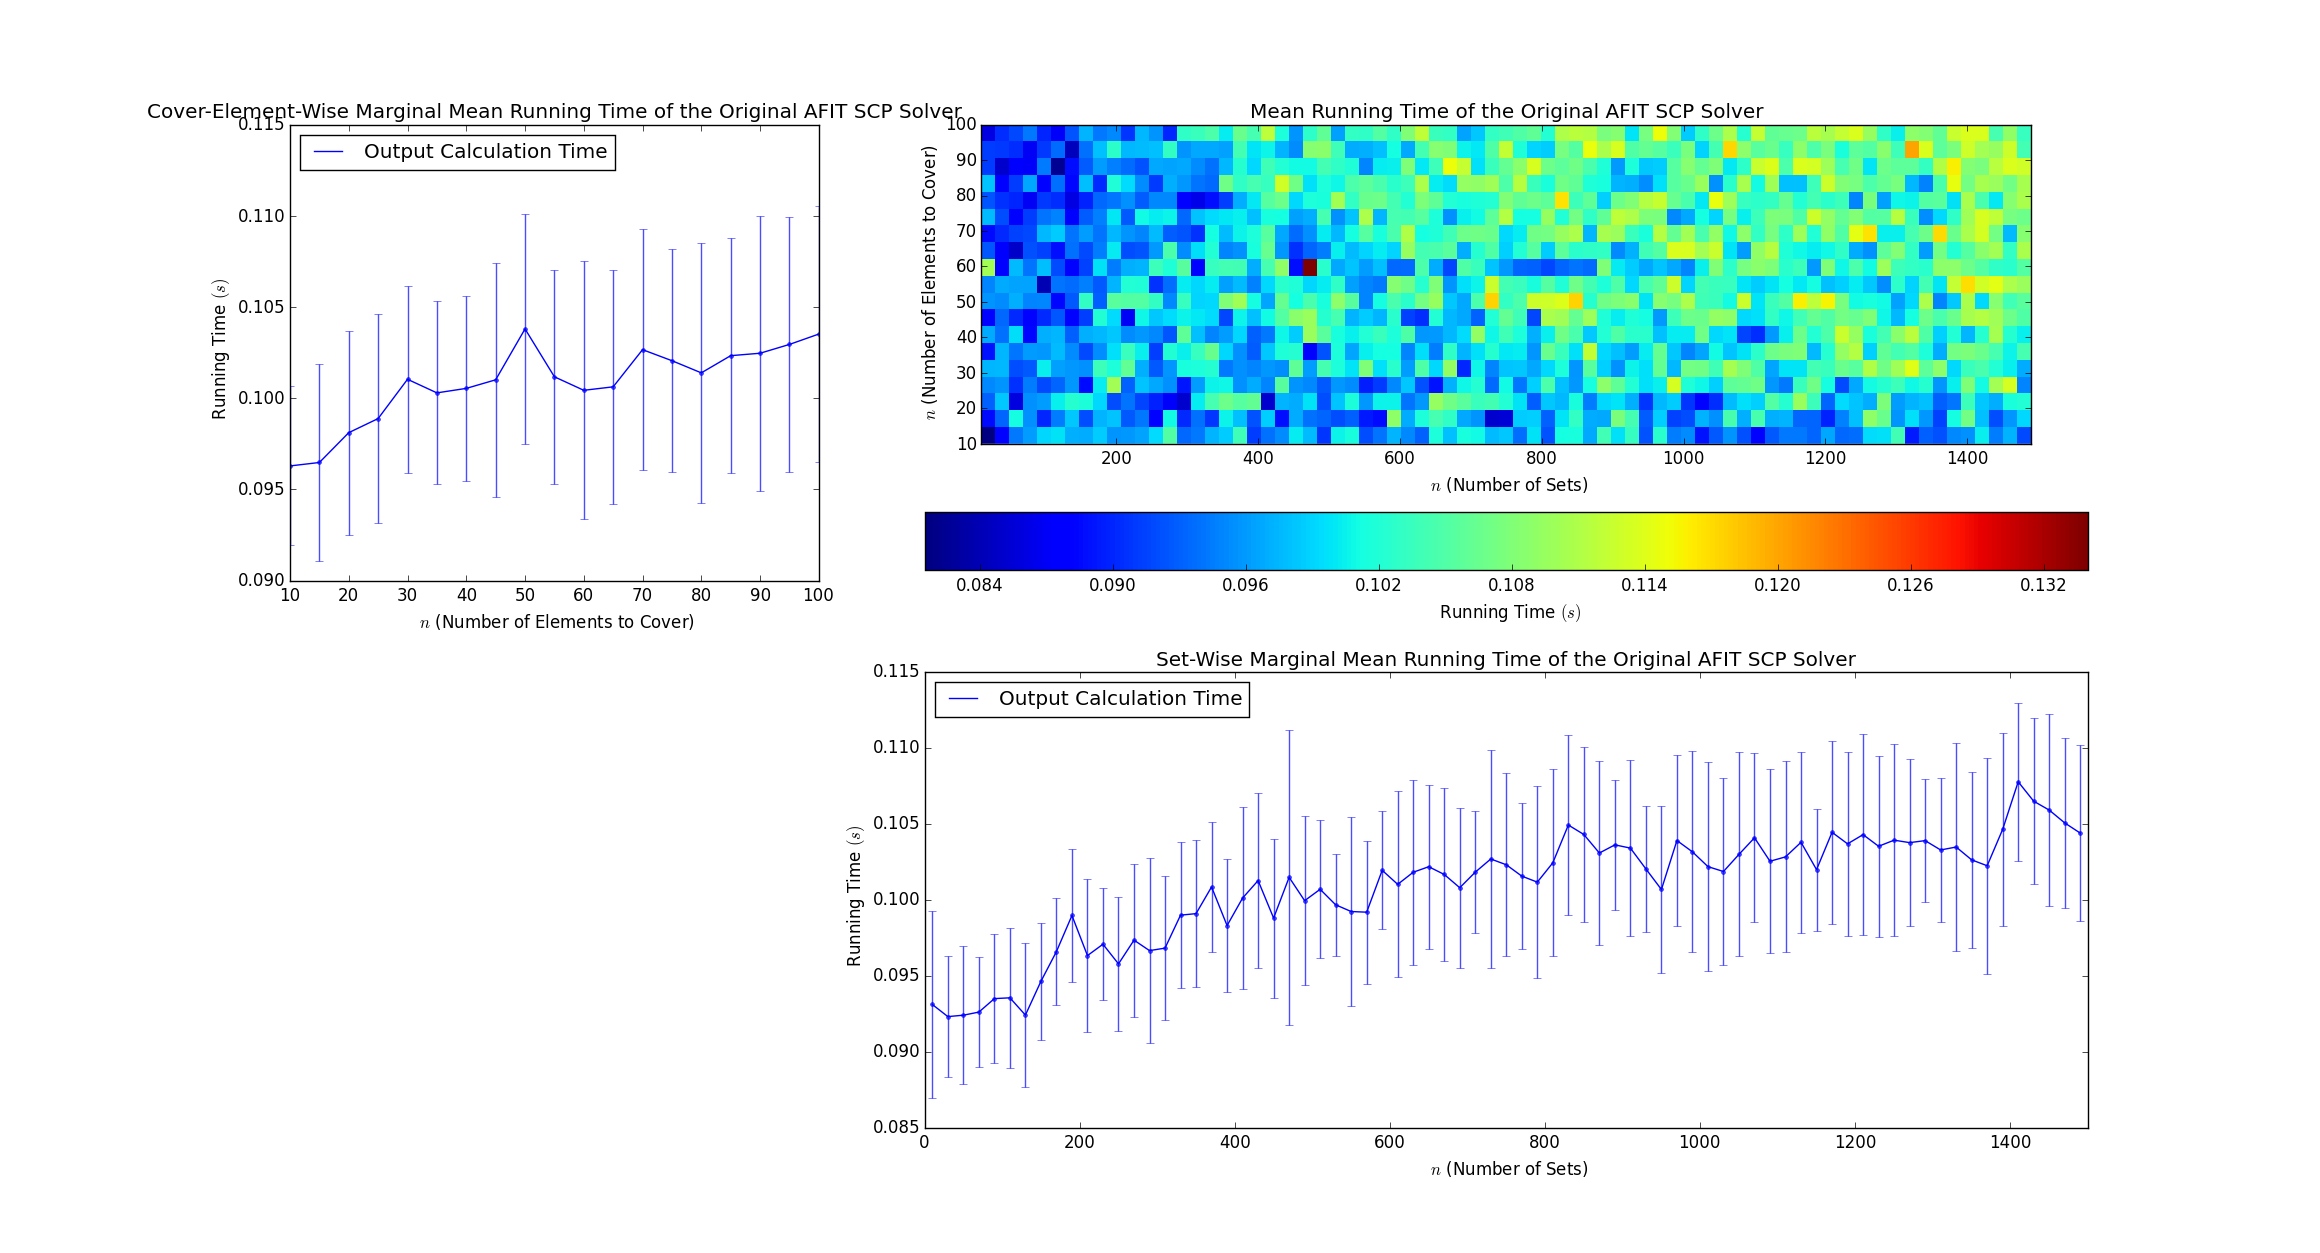
\includegraphics[width = 6.7in]{running_time_original_density0p3.png}}
		%  \vspace{2.0cm}
		\hfill
		
		%\vspace{-0.5cm}
		\caption{This figure displays the average running time performance of the original AFIT SCP Solver, over $20$ runs, for various instance configurations from the problem domain. All instances in this figure have a density of approximately $0.3$.}
		
	\end{figure}
	
	\begin{figure}[ht!]\label{fig:runtime_analysis_modified_density0p3}
		
		\centering
		\centerline{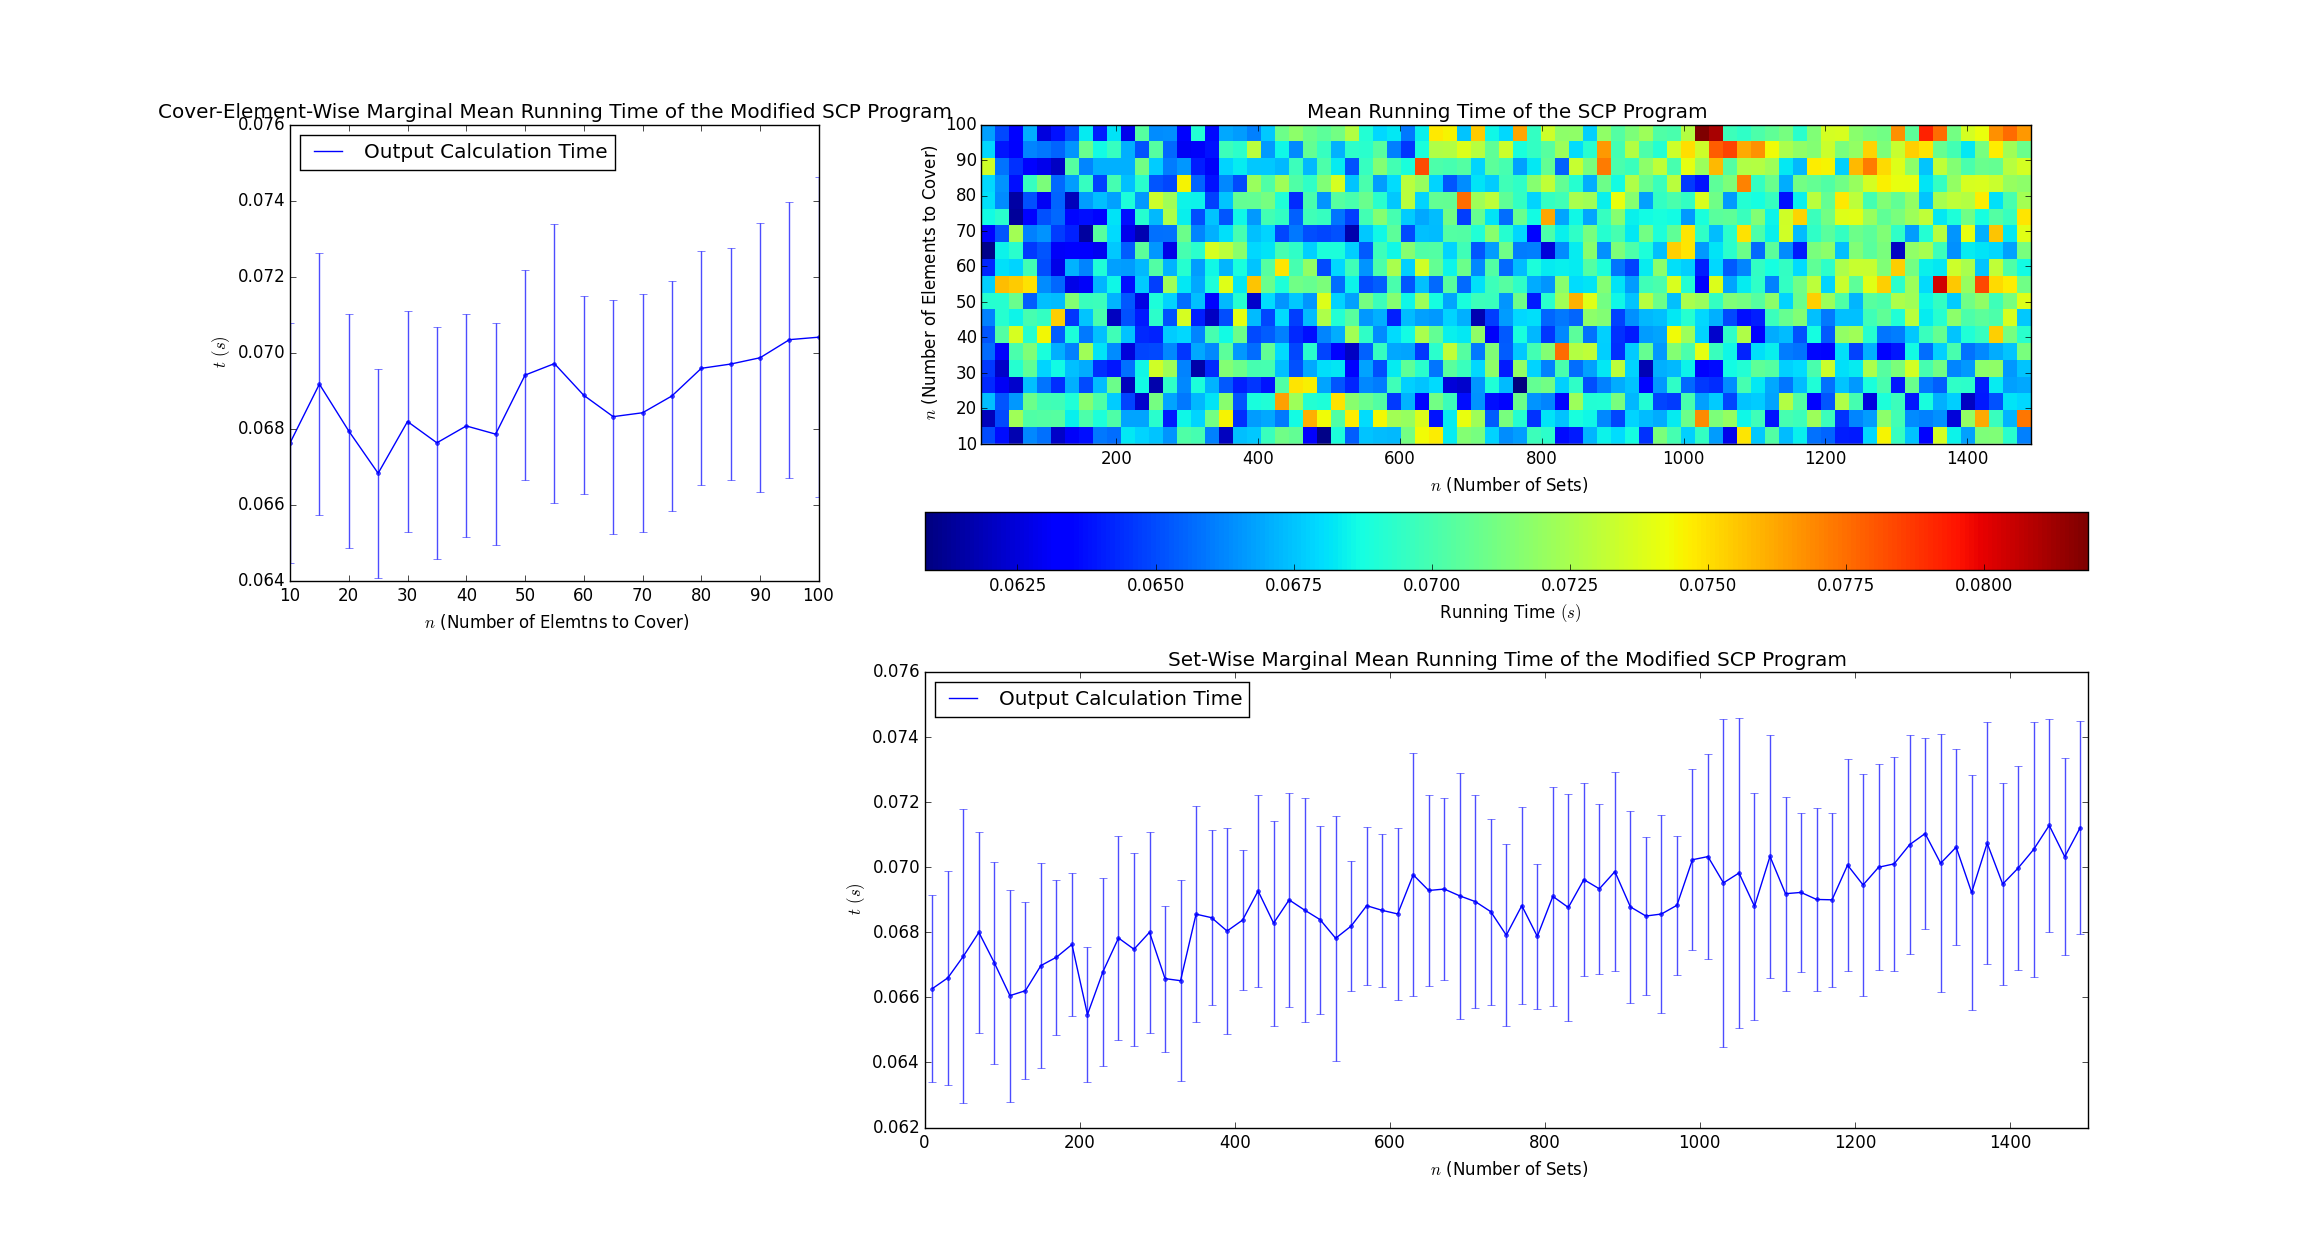
\includegraphics[width = 6.7in]{running_time_modified_density0p3_noout_noH1.png}}
		%  \vspace{2.0cm}
		\hfill
		
		%\vspace{-0.5cm}
		\caption{This figure displays the average running time performance of the modified AFIT SCP Solver, over $20$ runs, for various instance configurations from the problem domain. All instances in this figure have a density of approximately $0.3$.}
		
	\end{figure}
	
	\subsection{Search Tree [c.4]}
	
	A sample search tree is drawn below in figure \ref{fig:samplegraph}. The input elements are $\{1 2 3 4 5\}$, and the sets, defined in $(\{e_1,...,e_n\}, cost)$ format, are $(\{1, 3\},1)$,
	$(\{2, 3\},2)$,
	$(\{1, 4, 5\},3)$,
	$(\{2, 3, 5\},4)$,
	$(\{4, 5\}, 2)$.
	
	\begin{figure}[ht!] \label{fig:samplegraph}
		
		
		\centering
		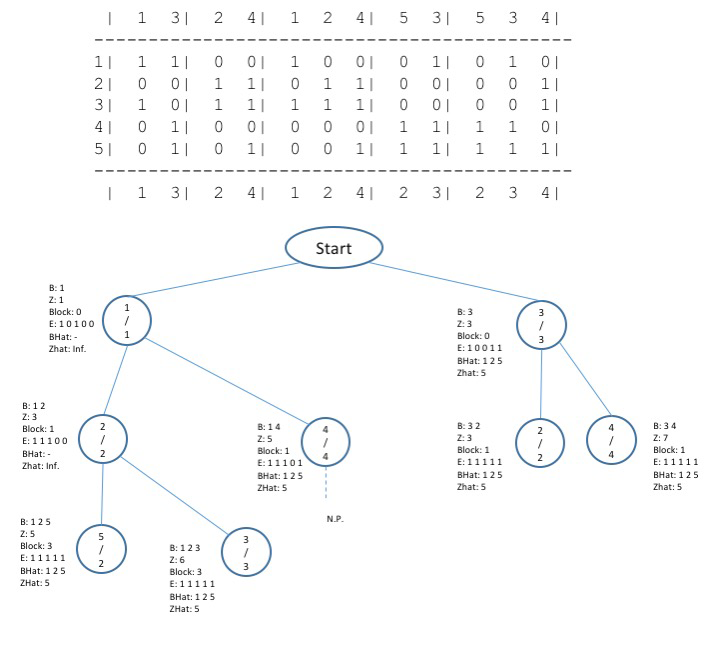
\includegraphics[width = 5.5in]{graph1.png}
		
		
		%\vspace{-0.5cm}
		\caption{This figure displays a sample graph created using the supplied input data. The initial Tableau is shown above the graph.}
		
		
	\end{figure}
	
	\section{AFIT SCP Program Software Engineering Practices} \label{scn:design}
	
	\subsection{SCP Implementation Discussion}
	\textit{Does the AFIT SCP Solver employ good software engineering practices?}
	Due to issues with both supplied code packages, we decided to write our own SCP solver from scratch. The decision to do this was based on the limited time available to solve the compilation issues, and a conscious decision to further understand the problem algorithm by implementing it. We did study the C++ implementation prior to creating our own solution, and it does follow many good software engineering principles, although from personal experience this evaluation can be subject to opinion. The code subscribed to valid object oriented design practices, was well documented, did not use unnecessarily complicated structures, although we could not identify an underlying design pattern. By dividing the work into small pieces, such as the list and block objects, it was simplifying the problem by the "divide and conquer" paradigm \cite{software}. We identified several instances of using functions to return multiple items with pointer references, which complicate the code somewhat. These variables probably should have been well labeled globals and used with caution. Because the code did not compile, I did examine the include structure of the files, and, as interpreted by the both Eclipse and Visual Studio, it appeared as if the software suffered from a "chicken or the egg" scenario where there was something of a circular dependency. This may have been eliminated with a more straight-forward order of object inheritance.
	
	Our own implementation was written in Java, using Eclipse IDE and Java 7, and there is no connection to the SCP solver 2006 Java code. We did not examine that software package. Instead, the algorithm was implemented as it was presented in by Christofides in section 4.3, \textit{A tree search algorithm for the SSP}, (modified according to Section 4.4). An advantage to this technique is that we obtained a greater understanding of the Christofides algorithm itself. We feel that this allowed us to better implement the heuristics.
	
	\textit{Discuss ease of understanding code in the AFIT SCP Solver. Discuss ease of standard interfaces.}
	
	The interfaces in the AFIT SCP C++ program were straight forward to understand. The set\_cover implements the main control structure of the algorithm, encapsulating steps 1 through 5 of the Christofides algorithm. Our implementation uses the searchSCP() function, which is very similar in control structure. Reductions are performed in reduction\_2\_1 and reduction\_2\_2, which are similarly performed in searchPossible, reduction 1 from section 4.2, and Heuristic 2, which is commented in SCPAlpha.java and implements reduction 2 from section 4.2. The C++ has several helper objects, such as List, opair, set, and block, with correspond to our own Block.java, Element.java, Tableau.java, and Set.java. We have an additional helper object to perform the sort, MergeSort.java. We believe that our own implementation has closer adherence to Object Oriented principles, however. Each of our objects directly correspond to a proposed data set in the design, and each is a simple extension of a standard ADT. The Block object is defined as $t$, the Tableau object is $T$, sets $S$ are defined in the Set Object, and an element $e \in E$ is implemented by the Element object. Additionally, our implementation uses the same data files as the C++ SCP implementation.
	
	
	\section{AFIT SCP Program Complexity} \label{scn:design}
	
	[Justin] Describe observed complexity.
	
	\section{Integration} \label{scn:design}
	
	
	
	\pagebreak
	\appendix		% Appendix begins here
	
	\section{Code Listing}
	
	\lstinputlisting[language=Java, caption=Main SCP Search Class]{SCPAlpha.java}
	\lstinputlisting[language=Java, caption=Element Class]{Element.java}
	%\lstinputlisting[language=Java, caption=Set Class]{Set.java}
	\lstinputlisting[language=Java, caption=Block Class]{Block.java}
	\lstinputlisting[language=Java, caption=Tableau Class]{Tableau.java}
	\lstinputlisting[language=Java, caption=Merge Sort Class Class]{MergeSort.java}
	
	
	\bibliographystyle{IEEEtran}
	\bibliography{algorthimBib}
	
\end{document}